% -*- root: ../mainThesis.tex -*-
\chapter{Further work}
%
There were several things that we were not able
to do due to either lack of time or simply because 
we were not able to solve the problem. Here we
list the most important things and provide some
information for further work.
%
\section{FieldOpt integration}
%
All functions need to be slightly adjusted so they
can be included into FieldOpt and integrated for
the optimization problem. The main reason is that
FieldOpt uses its own well and coordinate classes,
so we have to adjust the input and output format of
our code.
%
\section{Well length constraint projection}
%
The well length constraint projection only
handles wells that consist of a single straight line 
segment. There is no obvious extension of the 
current solution for non-straight wells. In the 
case of wells consisting of several connected 
straight lines there is an extension of our current algorithm
which is to only move the heel and toe along
the trajectory of the initial well. Extending
the lines beyond the initial lenght of the
well doesn't have a unique solution, since all
directions are feasible. This works 
perfectly well for wells consisting of multiple
line segments as long as the angles between the line 
segments are less than $45^\circ$.
%
\section{Inter-well distance constraint projection}
%
Note first that we were able to find one
case where our algorithm was not able to
solve the inter-well distance problem. This
is a simple case with two parallel shifted
line segments as shown in Figure \ref{fig:inter_well}.
%
\begin{figure}[H]
	\centering
	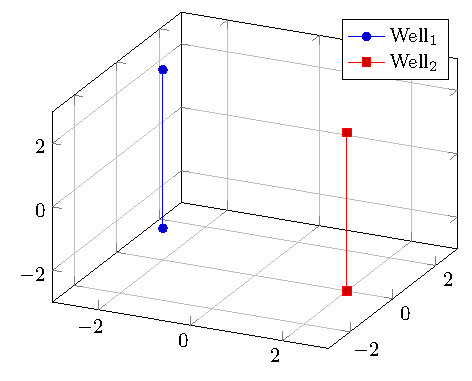
\includegraphics[width=0.80\textwidth]{figures/further_work/inter_well_distance.pdf}
	\caption{Well length projection on five wells. Five wells have been moved so that the well
										length constraint is satisfied for all wells.
										The inter-well distance constraint, however, is
										not satisfied.}
	\label{fig:inter_well}
\end{figure}
%
Several very similar cases were tried and
solutions were found for all of them. We
did not have time to resolve the problem
for this exact case, but we believe that 
the problem is due to numerical errors.
%
Every time we solve equation \eqref{eq:interwell_s}
there might be numerical issues when
computing the eigendecomposition of $A$.
Mathematically speaking there are no problems
involved in solving \eqref{eq:interwell_s}, but 
some care should be taken in these computations
to guarantee that a solution is found.
%
%
\section{Alternating projections}
%
The convergence of the alternating projection of well length
projection and inter-well distance projection was not proven.
From the results obtained for several wells it is reasonable 
to expect that the alternating projection will always converge.
The inter-well distance projection always moves pairs of wells
away from the average coordinate of their endpoints, whilst the
well length projection always leaves the average of the heel
and toe of a well unchanged. Because there was no spatial
restriction in our work, we hypothesize that the inter-well
distance projection will simply move points away from the
average of all the points until a solution is found.
Possible alternatives to the method of alternating projections, 
which might be worthwhile looking into, could be averaged 
projections \cite{Lewis_Luke_Malick_2} or Dykstra's projection
algorithm.
%